\documentclass[11pt,a4wide]{article}
\usepackage{verbatim}
\usepackage{listings}
\usepackage{graphicx}
\usepackage{a4wide}
\usepackage{color}
\usepackage{amsmath}
\usepackage{amssymb}
\usepackage[dvips]{epsfig}
\usepackage[T1]{fontenc}
\usepackage{cite} % [2,3,4] --> [2--4]
\usepackage{shadow}
\usepackage{hyperref}

\usepackage{subcaption}
%\setlength\parindent{0pt} % for å unngå indents
%\usepackage{parskip} %also to avoid indent, but with space

\setcounter{tocdepth}{2}

\lstset{language=c++}
\lstset{alsolanguage=[90]Fortran}
\lstset{basicstyle=\small}
\lstset{backgroundcolor=\color{white}}
\lstset{frame=single}
\lstset{stringstyle=\ttfamily}
\lstset{keywordstyle=\color{red}\bfseries}
\lstset{commentstyle=\itshape\color{blue}}
\lstset{showspaces=false}
\lstset{showstringspaces=false}
\lstset{showtabs=false}
\lstset{breaklines}

%\title{{\Huge {\bf Solving Schr\"odinger's equation for two electrons in a three-dimensional harmonic oscillator potential with a repulsive Coulomb interaction by using the Jacobi rotation algorithm}}\linebreak \small{Project 2, FYS-3150}}
%\author{Ina K. B. Kullmann}
%\date{\today}


%lager heftig forside:
\newcommand*{\titleAT}{\begingroup % Create the command for including the title page in the document
\newlength{\drop} % Command for generating a specific amount of whitespace
\drop=0.1\textheight % Define the command as 10% of the total text height

\rule{\textwidth}{1pt}\par % Thick horizontal line
\vspace{2pt}\vspace{-\baselineskip} % Whitespace between lines
\rule{\textwidth}{0.4pt}\par % Thin horizontal line

\vspace{0.5\drop} % Whitespace between the top lines and title
\centering % Center all text
\textcolor{black}{ % Red font color
{\Huge Solving Schr\"odinger's equation for two electrons in a three-dimensional harmonic oscillator potential with a repulsive Coulomb interaction by using the Jacobi rotation algorithm}\\[0.75\baselineskip] % Title line 1
%{\Large Tema:}\\[0.75\baselineskip] % Title line 2
%{\Huge Lydmåling og hørselstesting} % Title line 3
} 

\vspace{0.25\drop} % Whitespace between the title and short horizontal line
\rule{0.3\textwidth}{0.4pt}\par % Short horizontal line under the title
\vspace{0.25\drop} % Whitespace between the thin horizontal line and the author name

{\Large \textsc{Project 2, FYS-3150\\[0.75\baselineskip] \normalsize{Ina K. B. Kullmann}
}}\par % Author name

%\vfill % Whitespace between the author name and publisher text

\vspace{0.25\drop} % Whitespace between the title and short horizontal line
\rule{0.3\textwidth}{0.4pt}\par % Short horizontal line under the title
\vspace{0.25\drop} % Whitespace between the thin horizontal line and the author name

\begin{abstract}
The aim of this project is to numerically solve Schr\"odinger's equation for two electrons in a three-dimensional harmonic oscillator with a repulsive Coulomb interaction by using the Jacobi rotation algorithm. 

Before solving the problem for two electrons we will look at a simpler system, one electron in a three-dimensional harmonic oscillator potential. Then we will move on to the two electrons in a three-dimensional harmonic oscillator, but first without the Coulomb interaction. For each case we will reformulate the Schr\"odingers equation for this system to a dimentionless form and then to a descrete eigenvalue equation. This eigenvalue problem will we solve numerically with the Jacobi rotation algorithm and compare with the Armadillo library functions for the one electron system. 

The Jacobi rotation algorithm will be implemented numerically on a general form so that it can be applied to any eigenvalue problem with a symetrix matix. We will test the implementation of the Jacobi method on an arbitrary symetric matrix before moving on to solve the physical problems. 

When the procedure used on the two simplest cases are tested and understood we will apply the metods on the two electron system with a Coulomb interaction and plot the probability distrubution for different strengths of the interaction. 
\end{abstract}
\vspace*{0.25\drop} % Whitespace under the publisher text

\begin{center}
{ \scriptsize \noindent All source codes can be found at: \texttt{https://github.com/inakbk/Project\_2}. }
\end{center}

\rule{\textwidth}{0.4pt}\par % Thin horizontal line
\vspace{2pt}\vspace{-\baselineskip} % Whitespace between lines
\rule{\textwidth}{1pt}\par % Thick horizontal line

\endgroup}
%kode slutt for heftig forside


\begin{document}
%\maketitle
\titleAT % This command includes the title page





\newpage
\tableofcontents
\newpage

\section{Motivation and purpose}
Together with linear equations and least squares, the third major problem in matrix computations deals with the algebraic eigenvalue problem.\footnote{cite from \texttt{lectures2015} p. 225} It is therefore of great help to be able to solve eigenvalue problems numerically when we are dealing with large matices and complex systems. Such complex systems without any analytical solution occur often in physics.

Electrons confined in small areas in semiconductors, so-called quantum dots, form a hot research area in modern solid-state physics, with applications spanning from such diverse fields as quantum nano-medicine to the contruction of quantum gates. \footnote{cite from \texttt{lectures2015} p. 225} In this article we will study two electrons moving in a three-dimensional harmonic oscillator potential that repel each other via the Coulomb interaction. Throughout this paper we will assume spherically symmetry and let the angular momentum be $l=0$ (study the ground state only). 
  
For the numerical methods we have chosen to limit our attention to solving eigenvalue problems with symmetric matrices as meny problems can be written on this form. In particulary we focus on similarity transformations and the Jacobi rotation algorithm where we want to obtain both the eigenvalues and the eigenvectors for the systems. 


\newpage
\part{Theory}
\section{Numerical method}

First we will describe how similarity tansformations in general can be used to solve eigenvalue problems and then in detail how the Jacobi rotation algorithm solves this problem.

Let us assume that we have the eigenvalue problem 
\[
\bf A \bf x^{(v)} = \lambda \bf x^{(v)}
\]
where $\lambda^{(v)}$ are the eigenvalues and $\bf x^{(v)}$ the corresponding eigenvectors.\footnote{The introduction to this section is based on the lecturenotes"lectures2015.pdf"} Assuming that the matrix $\bf A$ is real and symetric we can use the Jacobi rotation algoritm to solve the eigenvalue problem. 

\subsection{Solving eigenvalueproblems using similarity transformations}
Let $\bf D$ be the diagonal matrix with the eigenvalues of $\bf A$ on the diagonal:

\begin{equation}
    \bf D = \left( \begin{array}{ccccccc} \lambda_1 & 0 & 0   & 0    & \dots  &0     & 0 \\
                                0  & \lambda_2 & 0 & 0    & \dots  &0     &0 \\
                                0   & 0 & \lambda_3 & 0  &0       &\dots & 0\\
                                \dots  & \dots & \dots & \dots  &\dots      &\dots & \dots\\
                                0   & \dots & \dots & \dots  &\dots       &\lambda_{n-1} & 0\\
                                0   & \dots & \dots & \dots  &\dots       &0 & \lambda_n

             \end{array} \right) 
      \label{eq:sematrix}
\end{equation} 

We say that a matrix $\bf B$ is a similarity transform of $\bf A$ if 
\[
\bf B = \bf {S^T AS}
\]
Where $\bf S$ is a unitary matrix so $\bf{S^TS} = \bf{S^{-1}S} = \bf I$\footnote{\texttt{http://mathworld.wolfram.com/UnitaryMatrix.html}}. The point of this is that the matrix $\bf B$ has the same eigenvalues as $\bf A$. Since $\bf A$ is real and symetric there exists a real orthonogal matrix $\bf S'$ such that: 
\[
\bf {S'^T AS'} = \bf D
\]
So the strategy is then to perform a series of similarity transformations on the original matrix $\bf A$ so that the matrix reduces to the diagonal matrix $\bf D$ with the eigenvalues on the diagonal:
\[
\bf{S_N^T\dots S_1^TAS_1\dots S_N} = \bf D
\]
where $\bf{S_1\dots S_N} = \bf S'$. This must be done on both sides of the equation. Only one transformation is given by:
\begin{align*}
(\bf{S^TAS})(\bf{S^Tx}) = \lambda \bf{S^Tx} \\
\bf{B(S^Tx)} = \lambda\bf{(S^Tx)}
\end{align*}
using that $\bf S$ is unitary. We see that the eigenvalue of $\bf B$ is the same as for $\bf A$, but the eigenvector is changed to $\bf{S^Tx}$.

\subsection{Jacobi's rotation algorithm} \label{sec:jacobi}
We will now see how we can find the eigenvalues of a real and symetric matrix $\bf A$ by using the Jacobi's rotation algoritm, or Jacobi's method.

The Jacobi's method introduces the ($n\times n$) unitary orthogonal transformation matrix 
\begin{equation}
    \bf S = \left( \begin{array}{ccccccc} 1 & 0 & 0   & 0    & \dots  &0     & 0 \\
                                0  & 1 & 0 & 0    & \dots  &0     &0 \\
                                0   & 0 & \cos \theta & 0  &0       &\dots & \sin \theta\\
                                0   & 0 & 0  & 1  &0       &\dots & 0\\
                                \dots  & \dots & \dots & \dots  &\dots      &\dots & \dots\\
                                0   & \dots & \dots & \dots  &\dots       &1 & 0\\
                                0   & \dots & -\sin \theta & \dots  &\dots       &0 & \cos \theta

             \end{array} \right) 
      \label{eq:sematrix}
\end{equation}
that performs a plane rotation around an angle $\theta$ in the Euclidean $n$-dimensional space. For simpler notation we define the quantities $\tan\theta = t= s/c$, with $s=\sin\theta$ and $c=\cos\theta$. The elements of the matrix $\bf S$ that differ from zero is given by the indexes $k,l$:
\[
s_{kk} = s_{ll} = c, \;\;\;\;  s_{kl} = -s_{lk} = -s,\;\; \;\;  s_{ii} = 1
\]
where $i\neq k$, $i\neq l$ and $i,j$ are the indexes of the matrix. Then the similarity transformation 
\[
\bf B = \bf {S^T AS}
\]
can be written on component form as:
\begin{align*}
b_{ii} &= a_{ii}\\
b_{ik} &= ca_{ik} - sa_{il} \\
b_{il} &= ca_{il} - sa_{ik} \\
b_{kk} &= c^2a_{kk} - s csa_{kl} + s^2 a_{ll} \\
b_{ll} &= c^2a_{ll} + 2csa_{kl} + s^2a_{kk} \\
b_{kl} &= cs(a_{kk} - a_{ll}) + (c^2 - s^2)a_{kl}
\end{align*}
We want to choose the angle $\theta$ so that all the non-diagonal matric elements becomes zero, that is $b_{kl} = 0$. Introducing a new variable $\tau$ dependent on $k,l$:
\begin{align*}
b_{kl} &= cs(a_{kk} - a_{ll}) + (c^2 - s^2)a_{kl} = 0\\
&\Rightarrow \frac{a_{ll}-a_{kk}}{a_{kl}} = \frac{c^2 - s^2}{cs} = \frac{2\cos{2\theta}}{\sin{2\theta}} = 2 \cot{2\theta}\\
&\Rightarrow \tau = \cot{2\theta} = \frac{a_{ll}-a_{kk}}{2a_{kl}}
\end{align*}
Then $b_{kl} = 0$ can be written as a second order equation
\begin{align*}
2\tau &= \frac{c^2 - s^2}{cs} = \frac{c^2}{cs} - \frac{s^2}{cs} = \frac{1}{t} - t\\
&\Rightarrow 2\tau t = 1 - t^2 \\
&\Rightarrow t^2 +2\tau t - 1 = 0\\
\end{align*}
with the solution
\[
t = -\tau \pm\sqrt{1 + \tau^2}.
\]
We obtain $c$ ans $s$ from
\begin{align*}
c^2 + s^2 = 1\\
\Rightarrow c = \frac{1}{\sqrt{1+t^2}},
\end{align*}
and using that $s=tc$.  

But which of the roots of $t$ should we choose? To make shure that the the similarity transformation does not make bigger changes to the other elements of $\bf A$ while making another element zero we minimize the difference between the matrices ${\bf B}$ and ${\bf A}$ by letting  $|\theta| \leq \pi /4$. This also makes shure that the iterations goes faster toward the solution, else the iterations might not converge at all after a reasonable number of iterations. 

Separating the inequality gives $\theta \leq \pi/4$ and $\theta \geq -\pi/4$. Starting with the first inequality:
\begin{align*}
\theta = \arctan t &\leq \pi/4 \\
t &\leq \tan (\pi/4) = 1
\end{align*}
and 
\begin{align*}
\theta = \arctan t &\geq -\pi/4 \\
t &\geq \tan(-\pi/4) = -1
\end{align*}
so we see that $|t| \leq 1\Rightarrow -\tau \pm \sqrt{1 + \tau^2} \leq 1$. If we look at the case where $\tau > 0$ and try the positive root of $t$ we see that:
\begin{align*}
-\tau + \sqrt{1 + \tau^2} &\leq -|\tau| + 1 + |\tau| = 1 \\
&\Rightarrow t \leq 1 \Rightarrow \theta \leq \pi/4
\end{align*}
must be satisfied.

If we then try the case when $\tau < 0$ and the negative root of $t$ we see that:
\begin{align*}
-\tau - \sqrt{1 + \tau^2} &= |\tau| - \sqrt{1 + \tau^2} \geq |\tau| - (1 + |\tau|) = -1 \\
&\Rightarrow t \geq -1 \Rightarrow \theta \geq -\pi/4
\end{align*}
must be satisfied. So the choice of the root of $t$ is dependent on $\tau$. When $\tau > 0$ we choose the positive root, and when $\tau< 0$ we choose the negative root to make shure that $|\theta| \leq \pi /4 $ is satisfied. \\~\\

The Jacobi algorithm can then be described as follows: 
\begin{enumerate}
\item Find the indexes $k, l$ of the maximum element of the matrix $\bf A$.
\item Obtain $c$ and $s$, the matrix elements of $\bf S$, given by $k, l$.
\item Calculate the similarity transformation $\bf{B = S^TAS}$.
\item Start on [1.] again, setting $\bf {A = B}$, untill all off-diagonal elements are esentially zero (less than a given threshold). When the iterations stop the eigenvalues are given by the matrix $\bf {D = B}$.
\end{enumerate}

We see that all information needed to perform a Jacobi rotation is given by the indexes $k, l$ of the maximum elements of $\bf A$.

\subsubsection*{Retriving the eigenvectors}
In this particular problem we also want to find the eigenvectors $\bf x^{(v)}$ of the matrix $\bf A$. The Jacobi's rotation method described in section \ref{sec:jacobi} does not return the eigenvectors. For every similarity transformation in the Jacobi's method the eigenvector is changed from $\bf x$ to $\bf{S^Tx}$. So it is possible to add a routine to the Jacobi's algorithm which ceeps track of the changes to the eigenvectors so that the eigenvectors can be returned when the iterations stop. The changes to the eigenvectors can be saved in a $n\times n$ matrix that is changed for every rotation. The matrix are initialized to the identity matrix and returns the eigenvectors on the columns when all the rotations are done. The returned eigenvectors are normalized. 

\section{One electron in a three-dimensional harmonic oscillator potential.}
We will first look at a simple system with known analytical solutions and later apply the methods obtained on a more complex system. First we need to write the Schr\"odinger's equation on a dimensionless form and then discretize the equation to solve it numerically. % to understand how to 

\subsection{Rewriting the Schr\"odinger's equation to a dimensionless form} \label{sec:rewrite_sch}
We look at the Sch\"odinger's equation for one electron at a radius $r\in [0,\infty)$ in a harmonic oscillator potential given by: 
\[
V(r)= (1/2)kr^2
\]
where $k=m\omega^2$ and $\omega$ is the oscillator frequence. The energy $E$ of the harmonic oscillator in three dimensions is given by:
\[
E_{nl}=  \hbar \omega \left(2n+l+\frac{3}{2}\right),
\]
with $n=0,1,2,\dots$ and $l=0,1,2,\dots$ is the orbital momentum of the electron. 

We are only interested in the solution of the radial part of the Schr\"odinger equation given by
\begin{equation}
  -\frac{\hbar^2}{2 m} \left ( \frac{1}{r^2} \frac{d}{dr} r^2
  \frac{d}{dr} - \frac{l (l + 1)}{r^2} \right )R(r) 
     + V(r) R(r) = E R(r).
     \label{eq:schr_1}
\end{equation}

We then use the substitution $R(r) = (1/r) u(r)$ and obtain
\[
  -\frac{\hbar^2}{2 m} \frac{d^2}{dr^2} u(r) 
       + \left ( V(r) + \frac{l (l + 1)}{r^2}\frac{\hbar^2}{2 m}
                                    \right ) u(r)  = E u(r) .
\]
The boundary conditions are $u(0)=0$ and $u(\infty)=0$.

We will modify equation \ref{eq:schr_1} further by introducing a dimensionless variable $\rho = (1/\alpha) r$ where $\alpha$ is a constant with dimension length and get
% 
\[
  -\frac{\hbar^2}{2 m \alpha^2} \frac{d^2}{d\rho^2} u(\rho) 
       + \left ( V(\rho) + \frac{l (l + 1)}{\rho^2}
         \frac{\hbar^2}{2 m\alpha^2} \right ) u(\rho)  = E u(\rho) .
\]
%
Now inserting $l=0$ and the rewritten potential $V(\rho) = (1/2) k \alpha^2\rho^2$ we obtain:
\[
  -\frac{\hbar^2}{2 m \alpha^2} \frac{d^2}{d\rho^2} u(\rho) 
       + \frac{k}{2} \alpha^2\rho^2u(\rho)  = E u(\rho) .
\]
and then multiply by $2m\alpha^2/\hbar^2$ on both sides
\[
  -\frac{d^2}{d\rho^2} u(\rho) 
       + \frac{mk}{\hbar^2} \alpha^4\rho^2u(\rho)  = \frac{2m\alpha^2}{\hbar^2}E u(\rho) .
\]
We fix the constant $\alpha$ so that
\[
\frac{mk}{\hbar^2} \alpha^4 = 1 \Rightarrow \alpha = \left(\frac{\hbar^2}{mk}\right)^{1/4}.
\]
and then define 
\[
\lambda = \frac{2m\alpha^2}{\hbar^2}E,
\]
Finally equation \ref{eq:schr_1} can be written as
\begin{equation}
  -\frac{d^2}{d\rho^2} u(\rho) + \rho^2u(\rho)  = \lambda u(\rho) .
  \label{eq: sch_1D_final}
\end{equation}
which is the equation we want to solve numerically. We know\footnote{This is given in the assignment text for Project 2, FYS3150..} that this equation has the eigenvalues $\lambda_0=3,\lambda_1=7,\lambda_2=11,\dots .$ for $l=0$. These analytical values will be used compare with the numerical solution in this one electron system.

\subsection{Discretizing the Schr\"odingers equation to solve the equation numerically.} \label{sec: descrete}
We will now rewrite the Schr\"odingers equation on a discretized form to be able to solve it as an matrix eigenvalue problem.

We use the expression for the second derivative of the function $u(\rho)$
\begin{equation}
    u''=\frac{u(\rho+h) -2u(\rho) +u(\rho-h)}{h^2} +O(h^2),
    \label{eq:diffoperation}
\end{equation} 
where $h$ is our step. We define the minimum and maximum values for the variable $\rho$,
$\rho_{\mathrm{min}}=0$  and $\rho_{\mathrm{max}}$ so that:
\[
  h=\frac{\rho_{\mathrm{max}}-\rho_{\mathrm{min}} }{n_{\mathrm{step}}}.
\]
where $n_{\mathrm{step}}$ is a given number of steps. Since $\rho \propto r$ and $r\in [0,\infty)$ the maximum value of $\rho$ should be $\rho_{\mathrm{max}}=\infty$. But we cannot set a infinite value when computing the solution numerically. We will therefore have to choose a significally large enough $\rho$.

We can then define an arbitrary value of $\rho$ as 
\[
    \rho_i= \rho_{\mathrm{min}} + ih \hspace{1cm} i=0,1,2,\dots , n_{\mathrm{step}}
\]
so that the Schr\"odinger equation for $\rho_i$ reads
\[
-\frac{u(\rho_i+h) -2u(\rho_i) +u(\rho_i-h)}{h^2}+\rho_i^2u(\rho_i)  = \lambda u(\rho_i),
\]
or in a more compact way with the harmonic oscillator potential $V_i=\rho_i^2$:
\begin{equation}
-\frac{u_{i+1} -2u_i +u_{i-1} }{h^2}+V_iu_i  = \lambda u_i,
\label{eq: sch_discrete_first}
\end{equation}
Then we can define first the diagonal matrix element
\[
   d_i=\frac{2}{h^2}+V_i,
\]
and the non-diagonal matrix element:
\[
   e_i=-\frac{1}{h^2}.
\]
We observe that in this case all the non-diagonal matrix element is given by a constant, so we can denote them all as $e=-\frac{1}{h^2}$ instead. 
 
With these definitions the Schr\"odinger equation (\ref{eq: sch_1D_final}) takes the following form
\begin{equation}
d_iu_i+e_{i-1}u_{i-1}+e_{i+1}u_{i+1}  = \lambda u_i,
\label{eq: sch_1d_descrete}
\end{equation}
where $u_i$ is unknown. This can be written as a matrix eigenvalue problem
\begin{equation}
    \left( \begin{array}{ccccccc} d_1 & e_1 & 0   & 0    & \dots  &0     & 0 \\
                                e_1 & d_2 & e_2 & 0    & \dots  &0     &0 \\
                                0   & e_2 & d_3 & e_3  &0       &\dots & 0\\
                                \dots  & \dots & \dots & \dots  &\dots      &\dots & \dots\\
                                0   & \dots & \dots & \dots  &\dots       &d_{n_{\mathrm{step}}-2} & e_{n_{\mathrm{step}}-1}\\
                                0   & \dots & \dots & \dots  &\dots       &e_{n_{\mathrm{step}}-1} & d_{n_{\mathrm{step}}-1}

             \end{array} \right)      \left( \begin{array}{c} u_{1} \\
                                                              u_{2} \\
                                                              \dots\\ \dots\\ \dots\\
                                                              u_{n_{\mathrm{step}}-1}
             \end{array} \right)=\lambda \left( \begin{array}{c} u_{1} \\
                                                              u_{2} \\
                                                              \dots\\ \dots\\ \dots\\
                                                              u_{n_{\mathrm{step}}-1}
             \end{array} \right) 
      \label{eq:sematrix}
\end{equation} 
This is the final equation that we will solve numerically. We will test the implementation of the problem by comparing with the analytical eigenvalues, but we are also interested in the eigenvector of the ground state so that we can plot the probability distrubution.

\section{Two electrons in a three-dimensional harmonic oscillator potential with Coulomb interaction.}
We will now study two electrons in a harmonic oscillator well which also interact via a repulsive Coulomb interaction.

We now rewrite the single-electron equation as
\[
  -\frac{\hbar^2}{2 m} \frac{d^2}{dr^2} u(r) 
       + \frac{1}{2}k r^2u(r)  = E^{(1)} u(r),
\]
where $E^{(1)}$ stands for the energy with one electron only. We then want to obtain a equation for the two electron system that is written on the same form as the one electron equation that we can solve numerically. First we look at the two electron syste without Coulomb interaction and we then add the interaction. Again we are only interested in the ground state with $l=0$. 

\subsection{The two electron system without Coulomb interaction}
The Schr\"odingers equation for two electrons in a harmonic oscillator potential with no Coulomb interaction can be written as
\begin{equation}
\left(  -\frac{\hbar^2}{2 m} \frac{d^2}{dr_1^2} -\frac{\hbar^2}{2 m} \frac{d^2}{dr_2^2}+ \frac{1}{2}k r_1^2+ \frac{1}{2}k r_2^2\right)u(r_1,r_2)  = E^{(2)} u(r_1,r_2) 
\label{eq: sch_2d_uC}
\end{equation}
with a two-electron wave function $u(r_1,r_2)$ and the two-electron energy $E^{(2)}$.

Since there is no electron interaction equation \ref{eq: sch_2d_uC} is separabel, it can be written as the product of two single-electron wave functions. We introduce the relative coordinate ${\bf r} = {\bf r}_1-{\bf r}_2$ and the center-of-mass coordinate ${\bf R} = 1/2({\bf r}_1+{\bf r}_2)$. With these new coordinates,  equation \ref{eq: sch_2d_uC} reads
\[
\left(  -\frac{\hbar^2}{m} \frac{d^2}{dr^2} -\frac{\hbar^2}{4 m} \frac{d^2}{dR^2}+ \frac{1}{4} k r^2+  kR^2\right)u(r,R)  = E^{(2)} u(r,R).
\]

We can separate this equation into equations for $r$ and $R$ since the wave function $u(r,R) = \psi(r)\phi(R)$ is a product. The energy is given by the sum of the relative energy $E_r$ and the center-of-mass energy $E_R$, that is
\[
E^{(2)}=E_r+E_R.
\]
For this article we will omit the center-of-mass energy in the calculations. Then the equation of interest becomes:
\[
\left(  -\frac{\hbar^2}{m} \frac{d^2}{dr^2}+ \frac{1}{4}k r^2\right)\psi(r)  = E_r \psi(r).
\]
By following the same approach as in section \ref{sec: descrete} equation \ref{eq: sch_2e_wCol} can written on a dimensionless form as:
\[
\left(  - \frac{d^2}{d\rho^2}+ \frac{1}{\rho}\right)\psi(\rho)  = \lambda\psi(\rho).
\]
We can then use equation \ref{eq:sematrix} to solve the problem numerically if the potential is replaced:
\[
V_i = \rho^2 \rightarrow V_i = \frac{1}{\rho}
\]
We will plot the probability distrubution to see if the results are reasonable before implementing the Coulumb interaction.

\subsection{The two electron system with Coulomb interaction}
We will now include the repulsive Coulomb interaction between two electrons. Introducing the term
\[
V(r_1,r_2) = \frac{\beta e^2}{|{\bf r}_1-{\bf r}_2|}=\frac{\beta e^2}{r},
\]
with $\beta e^2=1.44$ eVnm. With this extra term representing the interaction the $r$-dependent Schr\"odinger equation becomes
\[
\left(  -\frac{\hbar^2}{m} \frac{d^2}{dr^2}+ \frac{1}{4}k r^2+\frac{\beta e^2}{r}\right)\psi(r)  = E_r \psi(r).
\]

We want to manipulate this equation further to make it as similar as possible to the one electron equation (\ref{eq:schr_1}) we obtained earlier. Again we introduce the dimensionless variable $\rho = r/\alpha$ and repeating the same steps as in section \ref{sec:rewrite_sch}, we arrive at 
\[
  -\frac{d^2}{d\rho^2} \psi(\rho) 
       + \frac{1}{4}\frac{mk}{\hbar^2} \alpha^4\rho^2\psi(\rho)+\frac{m\alpha \beta e^2}{\rho\hbar^2}\psi(\rho)  = 
\frac{m\alpha^2}{\hbar^2}E_r \psi(\rho) .
\]
We manipulate this equation further by defining a 'frequency' which reflects the strength of the oscillator potential
\[
\omega_r^2=\frac{1}{4}\frac{mk}{\hbar^2} \alpha^4,
\]
and fix the constant $\alpha$ by requiring 
\[
\frac{m\alpha \beta e^2}{\hbar^2}=1
\]
or 
\[
\alpha = \frac{\hbar^2}{m\beta e^2}.
\]
Then defining 
\[
\lambda = \frac{m\alpha^2}{\hbar^2}E,
\]
so we finally can write the Schr\"odinger's equation as
\begin{equation}
  -\frac{d^2}{d\rho^2} \psi(\rho) + \omega_r^2\rho^2\psi(\rho) +\frac{1}{\rho} = \lambda \psi(\rho).
  \label{eq: sch_2e_wCol}
\end{equation}
We can again use equation \ref{eq:sematrix} to solve the problem numerically if the potential is replaced:
\[
V_i = \rho^2 \rightarrow V_i = w_r^2\rho^2 + \frac{1}{\rho}
\]

For specific oscillator frequencies, the above equation has answers in an analytical form found by M.~Taut\footnote{M.~Taut, Phys. Rev. A 48, 3561 - 3566 (1993).The article can be retrieved from the following web address \url{http://prola.aps.org/abstract/PRA/v48/i5/p3561_1}}. We will plot the probability distrubution for the cases $\omega_r = 0.01$, $\omega_r = 0.5$, $\omega_r =1$, and $\omega_r = 5$ for the ground state only ($l=0$).



\newpage
\part{Implementation, testing and finding the solutions of the Schr\"odinger equations}

\section{Implementation and testing of the Jacobi algorithm} \label{sec: test_jacobi}
\subsubsection*{Implementation}
The Jacobi rotation algorithm is structured into separate files which can be run once from \texttt{main.cpp} to solve one eigenvalueproblem. All files refered to in this section can be found in the folder \texttt{project\_2\_test\_jacobi} at: \\
\texttt{https://github.com/inakbk/Project\_2/tree/master/project\_2\_test\_jacobi}

The \texttt{jacobi.h} file contains all the routines for one rotation. The code finds the maximum element of the matrix, obtains the transformation matrix and does one rotation. The \texttt{jacobisolver.h} file does all the rotations for a given matrix $\bf B$ by calling the \texttt{jacobi.h} code and returns the eigenvalues and the first eigenvector. The parameter \texttt{tolerance} sets the limit of how small all the off diagonal elements in the matrix $\bf B$ needs to be before the rotations stop and the eigenvalues and the first eigenvector are returned. If the number of rotations (\texttt{numberOfIterations}) exceeds the maximum number of rotations (\texttt{maxNumberOfIterations}) before the off diagonal elements are smaller than the tolerance, the opreations are aborted with a warning message that the routine did not converge. The code also computes the execution time of all iterations for one matrix. 

We then see that the code in \texttt{jacobisolver.h} does the whole job of solving the eigenvalue problem with the Jacobi method and need only be given the matrix $\bf B$ with its dimension and the maximum number of iterations. Then the \texttt{main.cpp} program only needs to constructs the matrix $\bf B$ and call the \texttt{jacobisolver.h} code. With the help of \texttt{writetofile.h} the main program will write all parameters and the eigenvalues and eigenvectors to a file with filenames that distinguish the parameters that where run. These datafiles will then later be read by a python script and plot the data. 

\subsubsection*{Testing of the code}
Before using the Jacobi algorithm solve the physical problems the code was tested to make sure it worked properly. The purpose of the files in the folder \texttt{project\_2\_test\_jacobi} is to test the implementation of the Jacobi algorithm.

To do this the matrix $\bf B$ is initialized to a random symetric matrix. Then the solution is compared to the solutions generated by the \texttt{eig\_sym} function in the armadillo library.

To initialize $\bf B$ as a symetrix matrix we let $\bf C$ be a random matrix and set $\bf B = \bf{CC^T}$. Then $\bf B$ is a symetric matrix:
\[
\bf { B^T = (CC^T)^T = (C^T)^TC^T = CC^T = B}
\]
using that $\bf{ (ab)^T = b^Ta}$\footnote{\texttt{https://en.wikipedia.org/wiki/Transpose} (I dont have the mat1120 book here so wikipedia refrences it is then..)}. 

\section{Using the Jacobi rotation algorithm to solve the Schr\"odinger equations}

Equation \ref{eq:sematrix} is the matrix equation that we can use to solve both the one and two electron systems. The only difference between the systems are the potential $V_i$ and hence the matrix $\bf B$.

We can solve equation \ref{eq:sematrix} numerically using the Jacobi rotation algorithm as described in section \ref{sec: test_jacobi} by using the files \texttt{jacobisolver.h} and \texttt{jacobi.h} and \texttt{writetofile.h} to save the results. But in \texttt{main.cpp} the matrix would have to be initialized to the matrix in equation \ref{eq:sematrix}:
\[
\bf B = \left( \begin{array}{ccccccc} d_1 & e & 0   & 0    & \dots  &0     & 0 \\
                                e & d_2 & e & 0    & \dots  &0     &0 \\
                                0   & e & d_3 & e  &0       &\dots & 0\\
                                \dots  & \dots & \dots & \dots  &\dots      &\dots & \dots\\
                                0   & \dots & \dots & \dots  &\dots       &d_{n_{\mathrm{step}}-2} & e\\
                                0   & \dots & \dots & \dots  &\dots       &e & d_{n_{\mathrm{step}}-1}

             \end{array} \right)
\]
This is done in the folders \texttt{project\_2\_1e}, \texttt{project\_2\_2e} and \texttt{project\_2\_2e\_w\_col}\footnote{The reason the folders are separated are to not mix up the result files and be shure to be able to reproduce the results and look back if something is strange at a later point.} for respectively the one electron system and the two electron system without Coulomb interaction and with Coulumb interaction. The only difference between the folders are the potentials, or the matrix $\bf B$, the \texttt{.h} files are identical. The only exception is that the parameter $w_r$ is included in the last two electron case. 

But before the Schr\"odinger equations can be solved numerically the value of $\rho_{\mathrm{max}}$ and $n_{\mathrm{step}}$ that we will use needs to be decided.  

\subsection{Finding reasonable values for $\rho_{\mathrm{max}}$ and $n_{\mathrm{step}}$}

The matrix $\bf B$ is only dependent on the elements $d_i$ and $e$ which is only dependent on $\rho_{\mathrm{max}}$ and the dimension of the matrix $n_{\mathrm{step}}$. So which values of $\rho_{\mathrm{max}}$ and $n_{\mathrm{step}}$ should we choose? We need to test the algorithm so that we know which $\rho_{\mathrm{max}}$ that gives stable results and which values of $n_{\mathrm{step}}$ it is reasonable to use. 

First we have to decide which $\rho_{\mathrm{max}}$ to choose as this might affect the choice of $n_{\mathrm{step}}$. This can be done by looking at the first eigenvalues and choose the $\rho_{\mathrm{max}}$ which gives the smallest error when comparing to the analytical values. For the two electron case there are no analytical values to compare with so it is reasonable to choose a value which gives the most stable eigenvalues as a finction of  $n_{\mathrm{step}}$. We will therefore plot the eigenvalues as a function of $\rho_{\mathrm{max}}$.

Then we have to decide which precition of the eigenvalues we want to set a limit on how large $n_{\mathrm{step}}$ needs to be. This can be done by choosing a value of $n_{\mathrm{step}}$ that gives a small enough absolute error in the first three eigenvalues and that also have a reasonable execution time. We will plot the absolute error in the eigenvalues as a function of $n_{\mathrm{step}}$ to investigate this.

The execution time and precition is also related to how close to zero we force the off diagonal elements of $\bf B$ to be before reading off the eigenvalues. If the tolerance is too low we end up doing a lot of extra rotations that are very time consuming. We therefore should choose a tolerance that is low enough, but not too small. The number of transformations and the execution time will also be plotted as a function of $n_{\mathrm{step}}$.

When we are done deciding on the values of $\rho_{\mathrm{max}}$ and $n_{\mathrm{step}}$ the the Schr\"odinger equations can be solved numerically as described in the beginning of this section. 



\newpage
\part{Results and discussion}
\subsection*{The one electron system }
First the relative error between the three first numerical eigenvalues and the analytical eigenvalues where plotted as a function of $\rho_{\mathrm{max}} \in [3,6]$. This plot was generated for four different values of $n_{\mathrm{step}} \in [50, 100, 150, 200]$. 

In figure \ref{fig: p_max_big} we see that the absolute error decreases drastically as  $\rho_{\mathrm{max}}$ increases, here for $n_{\mathrm{step}}=100$, and does only increase sligtly after a minimum, for some of the eigenvalues. This was the case for all the plots for the different $n_{\mathrm{step}}$.

In figure \ref{fig: p_max_zoom} we see the plots with the four different $n_{\mathrm{step}}$ values zoomed in on the minimum for the error in the eigenvalues. We see that the minimum for the relative error reads different values of $\rho_{\mathrm{max}}$ for the eigenvalues and for different choice of $n_{\mathrm{step}}$. We see that for $n_{\mathrm{step}}=50$ the error in the eigenvalues are  large, $~0.01$ for the second eigenvalue. For $n_{\mathrm{step}}=100$ the error decreases to the half, given the same range of $\rho_{\mathrm{max}}$. 

The task is then to choose the value of $\rho_{\mathrm{max}}$ which gives the smallest error in all three eigenvalues combined. In every plot in figure \ref{fig: p_max_zoom} the point $(4.7, 0.0005)$ is marked. This is the point which gives the smallest absolute error in all of the eigenvalues for $n_{\mathrm{step}}=150$ and is the choice for $\rho_{\mathrm{max}}$ used in the numerical calculations. 

\begin{figure} [ht]
\centering
\includegraphics[width=0.7\textwidth]{plots_1e/p_max_n100_big.png}
\caption{This should be a very long caption text, but I am too lazy to write anything right now so I would please ask you to read the text that refers to this figure.}
\label{fig: p_max_big}
\end{figure}

\begin{figure} [htp]
\centering
		\includegraphics[width=0.6\textwidth]{plots_1e/p_max_n50_z.png}
		\includegraphics[width=0.6\textwidth]{plots_1e/p_max_n100_z.png}
		\includegraphics[width=0.6\textwidth]{plots_1e/p_max_n150_z.png}
		\includegraphics[width=0.6\textwidth]{plots_1e/p_max_n200_z.png}
\caption{This should be a very long caption text, but I am too lazy to write anything right now so I would please ask you to read the text that refers to these figures.}
\label{fig: p_max_zoom}
\end{figure}

To see if $n_{\mathrm{step}}=150$ is a wise choice we look at figure \ref{fig: abs.err_n} where the absolute error is plotted as a function of $n_{\mathrm{step}}$. In the top plot we see that the error decreases drastically as a function of $n_{\mathrm{step}}$ and is relatively small even for $n_{\mathrm{step}}=50$, but not for the three first eigenvalues at the same time. In the bottom plot we see that for $n_{\mathrm{step}}=150$ the error is maximum $~0.02$ and the effect of increasing $n_{\mathrm{step}}$ to 200 is small, the maximum error only decreases to $~0.01$.

\begin{figure} [htp]
\centering
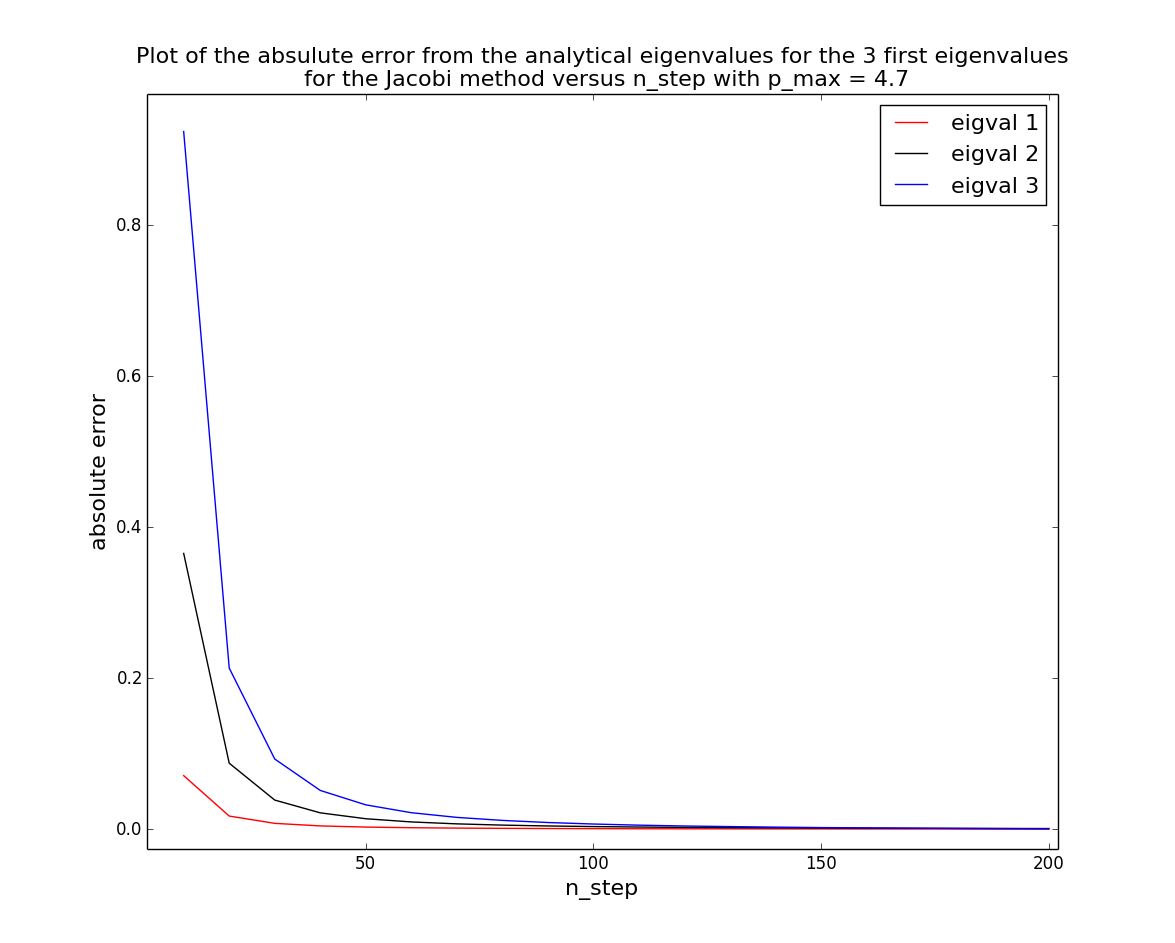
\includegraphics[width=0.8\textwidth]{plots_1e/abs_error.png}
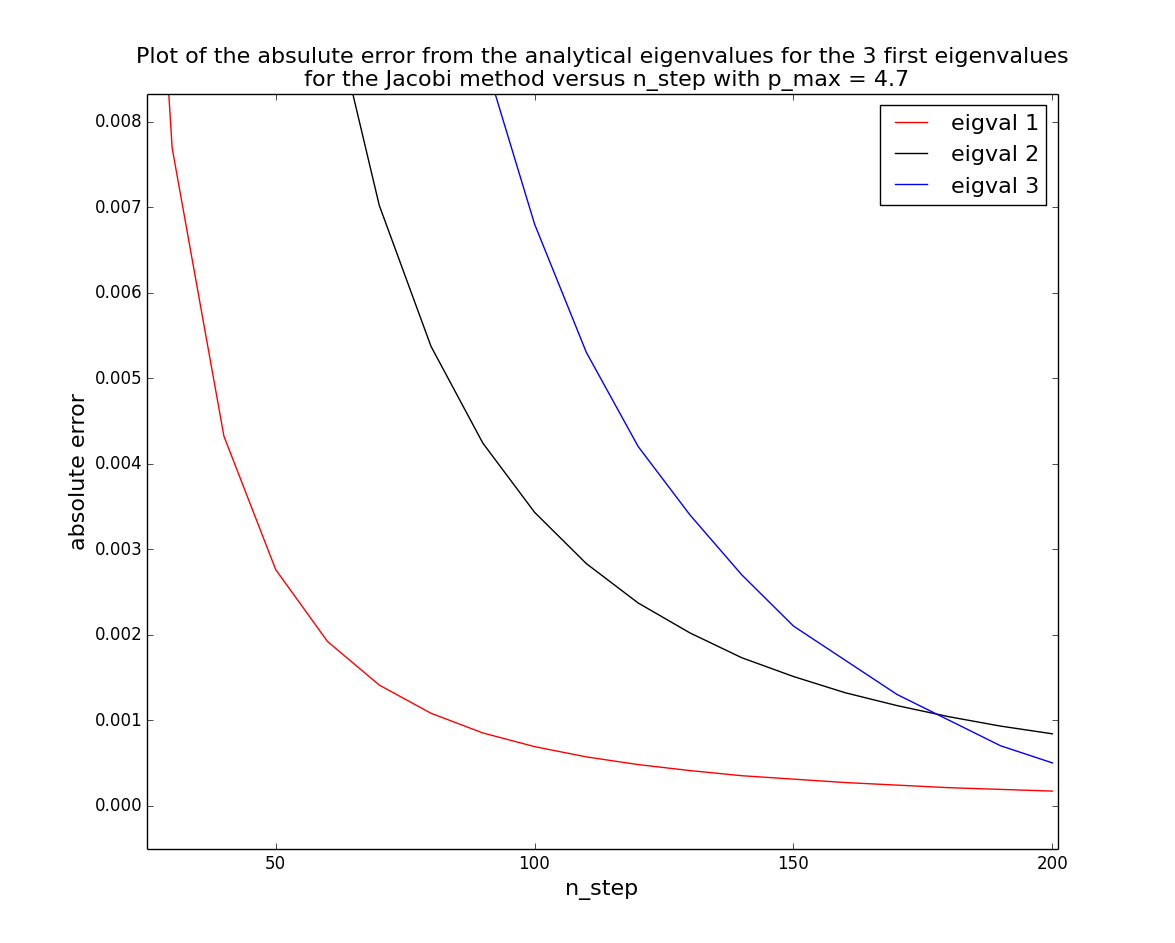
\includegraphics[width=0.8\textwidth]{plots_1e/abs_error_zoom.png}
\caption{This should be a very long caption text, but I am too lazy to write anything right now so I would please ask you to read the text that refers to this figure.}
\label{fig: abs.err_n}
\end{figure}

In figure \ref{fig: time} we see how the dimention of the matrix effects the execution time for the Jacobi method compared to the Armadillo library. We see that the execution time increases drastically as $n_{\mathrm{step}}$ is increased from 150 to 200. For the Jacobi method, while the Armadillo library apeares to use the same time for all values of  $n_{\mathrm{step}}$. The choice og $n_{\mathrm{step}}=150$ seems therefore reasonable. In figure \ref{fig: nr_iter} we see the number of iterations as a function of $n_{\mathrm{step}}$. We see that the number of iterations is more evenly increasing as a function of $n_{\mathrm{step}}$ than the execution time. 

\begin{figure} [htp]
\centering
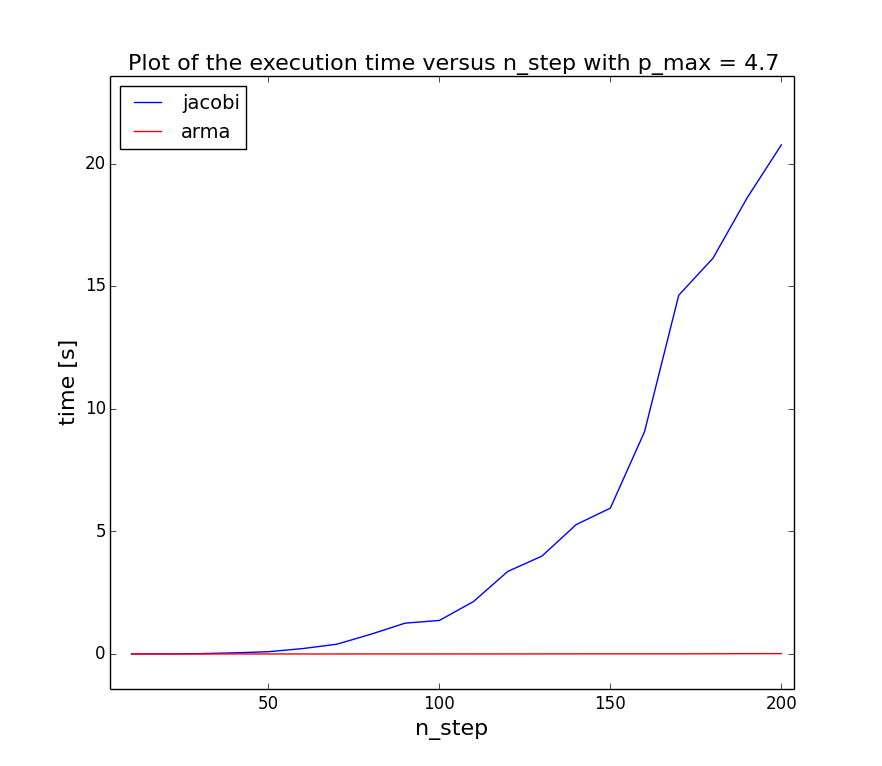
\includegraphics[width=0.7\textwidth]{plots_1e/time.png}
\caption{This should be a very long caption text, but I am too lazy to write anything right now so I would please ask you to read the text that refers to this figure.}
\label{fig: time}
\end{figure}

\begin{figure} [htp]
\centering
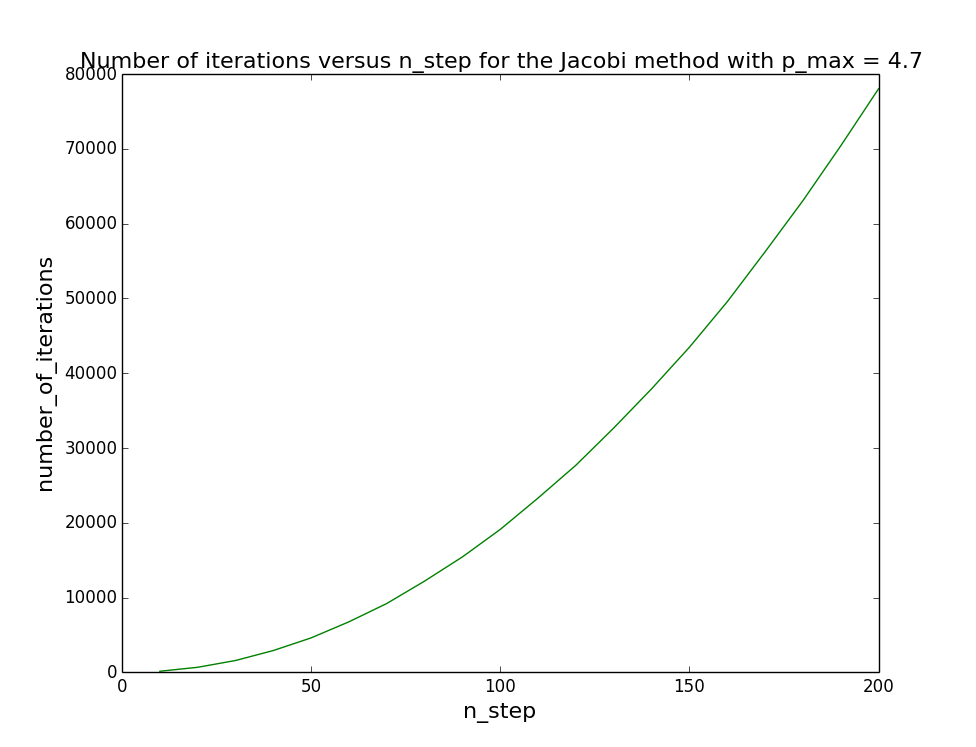
\includegraphics[width=0.7\textwidth]{plots_1e/nr_iterations.png}
\caption{This should be a very long caption text, but I am too lazy to write anything right now so I would please ask you to read the text that refers to this figure.}
\label{fig: nr_iter}
\end{figure}

Finally in figure \ref{fig: prob_1e} we see the probability distribution, the eigenvector for the ground state squared plotted as a function of the dimensionless position $\rho$.

\begin{figure} [h!]
\centering
\includegraphics[width=\textwidth]{plots_prob/prob_1e.png}
\caption{noe langt}
\label{fig: prob_1e}
\end{figure}

\section*{The two electron system}
In figure \ref{fig: prob_2e_w_col} we see the value of the first, second and the third eigenvalue plotted as a function of $\rho_{\mathrm{max}}$ where each line in the plot corresponds to a value of $n_{\mathrm{step}}$. We wish to choose a value for $\rho_{\mathrm{max}}$ so that the results for the eigenvalues are stable as a function of $n_{\mathrm{step}}$. If we discard $n_{\mathrm{step}}=50$ we see that as long as we choose a value of $\rho_{\mathrm{max}}$ larger than $~5$ the values of the first, second and third eigenvalue are independent on the choice of $n_{\mathrm{step}}$. Therefore $n_{\mathrm{step}}=150$ and $\rho_{\mathrm{max}}=6$ seems like a reasonable choice.

\begin{figure} [ht]
\centering
\includegraphics[width=0.6\textwidth]{plots_p_max_2e/1eigval.png}
\includegraphics[width=0.6\textwidth]{plots_p_max_2e/2eigval.png}
\includegraphics[width=0.6\textwidth]{plots_p_max_2e/3eigval.png}
\caption{This should be a very long caption text, but I am too lazy to write anything right now so I would please ask you to read the text that refers to this figure.}
\label{fig: p_max_2e_w_col}
\end{figure}

The final desired result, the probability distribution for the interaction two electron system is plotted in figure \ref{fig: prob_1e}. The eigenvector for the ground state squared plotted as a function of the dimensionless position $\rho$ for different values of the strength of the Coulumb interaction $w_r$. We see that the shape of the distribution changes for the different values of $w_r$. 

\begin{figure} [ht]
\centering
\includegraphics[width=\textwidth]{plots_prob/prob_2e_w_col.png}
\caption{This should be a very long caption text, but I am too lazy to write anything right now so I would please ask you to read the text that refers to this figure.}
\label{fig: prob_2e_w_col}
\end{figure}

\section*{Discussion and Experiences}

This problem has been both fun and frustrating to work with. It was very hard to get a owerview of the problem and a lot of time was spent on details that was not even useful for the problem. It was frustrating to 'blindfoldedly' looking for the values of $n_{\mathrm{step}}$ and $\rho_{\mathrm{max}}$ as i did not know what to expect. 

The results generated for the one electron system was as expected, the solutions are already known analytically. But it was quite unexpected to see that the execution time for the Jacobi method incrased so rapidly and that the execution time for the  Armadillo library did not. Later realizing that this is because the tolerance was once set to a very low value for testing, but forgotten to reajust again. So the value of the tolerance was set to $10^-14$ instead of $10^-8$ and this have affected the results. It would have been interesting to rerun and see if the execution time and number of iterations for the Jacobi method did change, but there was no time to do this. The Armadillo code must also have a very fast algorithm, or something have gone wrong in my routines when obtaining the execution time. 

It was very satisfying to finally obtain the plot of the probability distribution for the interacting two electron system! But very frustrating to have nothing to compare with, only a insecure gut feeling that the results seems reasonable and physical. 

I have also used to much time on this project, but I have learned a lot that will be useful for the next projects!

\end{document}





